\documentclass[resume]{subfiles}


\begin{document}
\section{Valgrind}

\subsection{Outils de Valgrind}
\begin{itemize}
\item Memcheck : Détection d'erreur mémoire
\item Cachegrind : Profiler de mémoire cache
\item Callgrind : Profiler de cache avec infos supp et graph
\item Helgrind : Détection d'erreur de threads 1
\item DRD : Détection d'erreur de threads 2
\item Massif : Profiler de heap et stack (memory leak)
\item DHAT : Profiler de bloc dans le heap
\end{itemize}

\subsection{Utilisation des outils}
\begin{figure}[H]
    \centering
    \includegraphics[width=0.9\columnwidth, page=2]{Schemas-crop.pdf}
\end{figure}

\subsection{Trouver le bon outil}
L'outil Memcheck regroupe beaucoup de fonctionnalité. C'est lui qu'il faut utilisé en priorité

\end{document}